\documentclass[11pt]{article}
\usepackage{graphicx}
\usepackage{amssymb}
%\usepackage[nomarkers]{endfloat}
\usepackage{natbib}
\usepackage{setspace}
\usepackage{wasysym}
\usepackage{wrapfig}

\textwidth = 7 in
\textheight = 9 in
\oddsidemargin = -0.5 in
\evensidemargin = -0.5 in
\topmargin = 0.0 in
\headheight = 0.0 in
\headsep = 0.0 in
\parskip = 0.1in
\parindent = 0in
\renewcommand{\Pr}{\mathbb{P}}
\usepackage{paralist}
\usepackage{url}
\newcommand{\href}[2]{\url{#2}}
\usepackage{hyperref}
\hypersetup{backref,   linkcolor=blue, citecolor=red, colorlinks=true, hyperindex=true}
\begin{document}
notes from the week of Feb.~18, 2019 \\
\tableofcontents

We worked through Bayes' rule and then talked about the difference
between confidence intervals and Bayesian posterior probability
statements (see \url{http://phylo.bio.ku.edu/biostats/bad_bean_counter.pdf})

\section{Posterior distribution for $\nu$}.
We'll use $\nu = ut$, as the branch length in terms of the expected number of changes
    over a branch in a genealogy.

Back to our original example $X=5$ and the branch length from JKK to the MRCA and back to 
you is $2\nu$.

We assume that the Poisson describes the probability of any number of mutations given
    the expected number
In an ML context, you'd get $\hat{\nu} = 2.5$ and you could define a 95\% confidence interval
    based on what values of $\nu$ give you log-likelihoods that are 1.92 lower than
    the log-likelihood at $\nu = 2.5$.

For a Bayesian inference of $\nu$, we start with Bayes' rule applied to this problem:
\begin{eqnarray}
f(\nu\mid X=5) = \frac{g(\nu)\Pr(X=5\mid \nu)}{\Pr(X=5)}
\end{eqnarray}
where $f(\nu\mid X=5)$ is the ``posterior probability density of $\nu$'' and
$g(\nu)$ is the ``prior probability density of $\nu$.''
Both are probability distributions, meaning that the integral
of the density over
the feasible range for $\nu$ (which is $0\leq\nu < \infty$) will be 1.

\subsection{the prior}
In a purely subjective Bayesian perspective we'd have to figure out
    how to describe our prior beliefs.
In practice, we often pick an analytically tractable distribution
    that is close to what we want to express as our prior beliefs, while
    still being easy to work with mathematically.

Last week we saw that population genetics tells us the $t\sim\mbox{ Exponential}(\lambda=1/N)$ where $N$ is the effective population size.
If we pretended that we knew the mutation rate for our locus (which
is not terribly implausible as there is a lot of data about the rate
of molecular evolution in mammalian mitochondrial genes), then
perhaps our uncertainty about $\nu$ can be thought of as being 
basically some exponential distribution.

An exponentail distribution is just a special case of a Gamma distribution,
where $\alpha=1$ and $\beta=\lambda$ when we are using the ``shape+rate'' parameterization of the \href{https://en.wikipedia.org/wiki/Gamma_distribution}{the Gamma distribution}.
Wikipedia tells us that if $x\sim \mbox{Gamma}(\alpha, \beta)$ then:
\begin{eqnarray}
g(x \mid \alpha, \beta) &=& \frac{\beta^{\alpha}}{\Gamma(\alpha)}x^{\alpha - 1}e^{-\beta x} \\
\mathbb{E}[x] & = & \frac{\alpha}{\beta} \\
\mbox{Var}(x) & = & \frac{\alpha}{\beta^2}
\end{eqnarray}


So if we wanted to say our prior on $\nu$ is a fairly broad exponentail
    distribution with a mean of 5 ($\lamba=\frac{1}{5}=0.2$ in the typical Exponential
    notation or $\alpha=1,\beta=.2$ in our preferred notation for the Gamma).
So, to be concrete:
\begin{eqnarray}
g(\nu \mid \alpha, \beta) &=& \frac{\beta^{\alpha}}{\Gamma(\alpha)}\nu^{\alpha - 1}e^{-\beta\nu} \\
g(\nu \mid \alpha=1, \beta=0.2) &=& \frac{0.2}{\Gamma(1)}\nu^{0}e^{-0.2\nu} 
\end{eqnarray}

\subsection{the likelihood}
Recall that our expectated number of mutations in $\2\nu$ and our likelihood is Poisson:
\begin{eqnarray}
\Pr(X=5\mid \nu) &= & \frac{(2\nu)^5e^{-2\nu}}{5!}
\end{eqnarray}

\subsection{the marginal likelihood}
The denominator of Bayes' rule is tough it is:
\begin{eqnarray}
\Pr(X=5) &= &\int_0^{\infty} \Pr(X=5\mid \nu)g(\nu) d\nu
\end{eqnarray}
Crucially it is is a constant -- it is the same for every value of $\nu$.
So we'll just call it $K$

\subsection{the posterior}
So what is our posterior density?
\begin{eqnarray}
f(\nu\mid X=5) & = & \frac{g(\nu)\Pr(X=5\mid \nu)}{\Pr(X=5)} \\
& = & \frac{\frac{0.2}{\Gamma(1)}\nu^{0}e^{-0.2\nu}\frac{(2\nu)^5e^{-2\nu}}{5!}}{K}\\
& = & K_2 \nu^{0}e^{-0.2\nu}\nu^{5}e^{-2\nu} \\
& = & K_2 \nu^{5}e^{-2.2\nu}
\end{eqnarray}
where $K_2$ is a constant that is just a product of all of the parts of
the equation that don't depend on $\nu$.

The key thing to recognize is that the shape of the density is just
    the relative height as $\nu$ changes.
That shape is determined by $\nu^{5}e^{-2.2\nu}$
$K_2$ is the ``normalization constant'' that we'd have to multiple to 
    every density so that the whole thing integrates to 1.
Conveniently, the shape of the posterior that we derived is 
    exactly the shape of a Gamma$(\alpha=6, \beta=2.2)$ distribution.
That means that $K_2=2.2^6/\Gamma(6)$ (because that is the coefficient
of the Gamma density, and the Gamma integrates to 1, too).
Figure \ref{plp} shows the prior, likelihood, and posterior for $\nu$

\begin{figure}[h]
\hskip-1cm 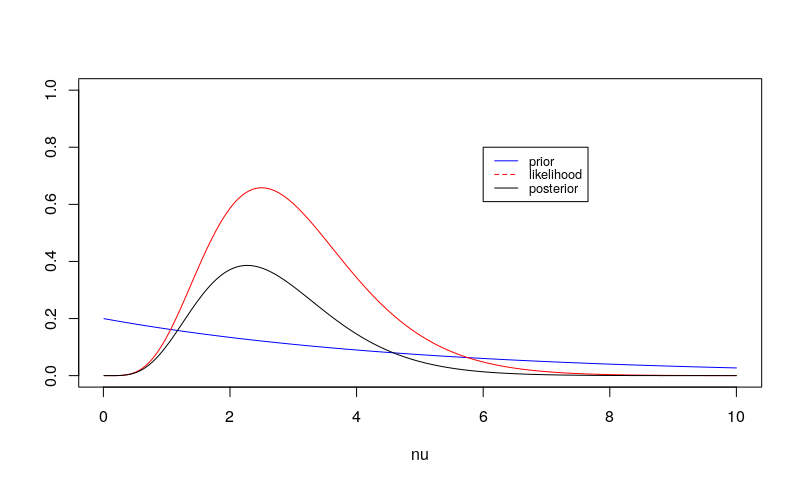
\includegraphics[scale=1]{images/poisson-gamma-conjugacy.png}
\caption{Poisson likelihood (red - not a probability distribution over $\nu$),
the Gamma$(\alpha=1, \beta=0.2)$ prior and Gamma$(\alpha=6, \beta=2.2)$}\label{plp}
\end{figure}

\subsection{a 95\% credible interval}
Because the posterior is a nice analytically well-characterized distribution,
we can use {\tt qgamma(0.025, shape=6, rate=2.2)} and {\tt
qgamma(0.975, shape=6, rate=2.2)}
in R to find the values of $\nu$ that chop off the lower 
and upper 2.5\% tails to get a
credible interval.
Most Bayesians use a slightly different Highest Posterior Density (HPD)
interval, which is the smallest interval (on the $\nu$ axis) that integrates
to 0.95.
But these intervals would be quite similar for this problem.

Figure \ref{cis} shows the likelihood with the 1.92 log drop (the maximized likelihood divided by $e^{1.92}$).
The ML-based 95\% confidence interval is $0.87 < \nu <5.37$, while
the Bayesian 95\% credible interval produces by cropping off 2.5\%
from each tail is the statement that $\Pr(1.00<\nu<5.30 \mid X=5) = 0.95$
using our prior.

It is common for the 95\% credible interval to be a tiny bit smaller (more
precise) than the 95\% confidence interval.
Recall that the confidence interval is based on a recipe guaranteeing
    95\% coverage that was designed before we look at the data.
By fully exploiting prior information and conditioning our inference fully
on the data, the Bayesian approach has a bit more power (at the cost of 
having more inputs that it could be sensitive to).

\begin{figure}[h]
\hskip-1cm 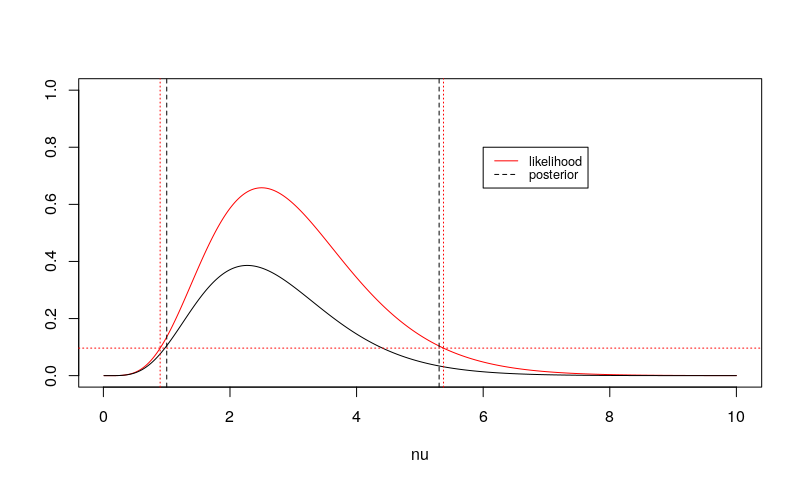
\includegraphics[scale=1]{images/dueling-cis.png}
\caption{Likelihood and posterior. Confidence interval boundaries computed
by the 1.92 $\ln$-likelihood drop method. Credible interval boundaries
computed by the {\tt qgamma} method in R. }\label{cis}
\end{figure}
\end{document}

\section{Revisiting the time to MRCA from mutation counts}
\subsection{the data}
Now we'll add my sequence to the previous example.
We have a tree with 1 or 2 MRCAs.
Our data is
$X=[3,2,6]$,
so our sample size is $n=3$.

\section{the likelihood}
Given that we have worked on similar problems recently, we probably would reach
for the Poisson likelihood:
\begin{eqnarray}
\Pr(X\mid ut_1, ut_2, ut_3)& = & \prod_{i=1}^{n} \Pr(x_i\mid ut_i)\\
& = & \prod_{i=1}^{n} \frac{(ut_i)^{x_i}e^{-ut_i}}{x_i ! }
\end{eqnarray}
This is not wrong, but it fails to accurately convey the constraints on the parameter.
If you and JKK share a mitochondrial MRCA more recently than either of you do with me, then $t_1=t_2$ and $t_3> t_1$.

We can express those constraints on the parameters mathematically as an expression of the domain.
In this case: 
\begin{eqnarray}
    t_1, t_2, t_3, u & \in &  \mathbb{R}\\
    0 & < u < & \infty\\
    0 & < t_1 < & \infty\\
    t_1 & = & t_2 \\
    t_1 & \leq & t_3
\end{eqnarray}
where the first line says that all four parameters are real numbers (not integers, 
not complex numbers, {\em etc.}), and then the equations and inequalities constrain
the feasible range of them.

This is fine and it works fine.

Sometimes it is easier to reparameterize in a way that makes the parameters more
``orthogonal'' (in some vague sense).
What occurs to me is to use $\omega$ to represent a mutation-rate-scaled waiting
time to the previous coalescence event.
That occurs to me because it is the kind of thing we often do in coalescent theory.
It may not occur to you, and that is OK -- you can get the right answers without
this reparameterization.

Specifically:
\begin{eqnarray}
    \omega_1, \omega_2 & \in &  \mathbb{R}\\
    0 & < \omega_1, \omega_2 < & \infty\\
     ut_1 = ut_2 & = & 2\omega_1  \\
    ut_3 &= & 2\omega_2 + \omega_1
\end{eqnarray}


\begin{eqnarray}
\Pr(X\mid \omega_1,\omega_2)& = & \prod_{i=1}^{n} \Pr(x_i\mid \omega_1,\omega_2)\\
& = &
 \frac{(2\omega_1)^2e^{-\omega_1}(2\omega_1)^3e^{-\omega_1}\left(\omega_1+2\omega_2\right)^6e^{-(\omega_1+2\omega_2)}}{2!3!6!} \\
& = & \frac{2^2 2^3}{2!3!6!}\left[\omega_1^5e^{-2\omega_1}\right]
\left[\left(\omega_1+2\omega_2\right)^6e^{-(\omega_1+2\omega_2)}\right] \\
\ln L & = & 5\ln(2)-\ln(2!3!6!)+ \left[5 \ln(\omega_1) -2\omega_1\right] +
\left[6\ln\left(\omega_1+2\omega_2\right) -\omega_1- 2\omega_2)\right] 
\end{eqnarray}
where the [] braces just help us see that the likelihood is coming from 2 paths in the tree: the one between JKK and you $x_1+x_2 = 5$ and the one that says that MTH
is 6 mutations away from that common ancestor $x_3 = 6$

You can derive how $\hat{\omega_1}=2.5$ based soley on $x_1+x_2 = 5$.
However it is not clear if that is actually the maximum likelihood
if we use all the data (and we should always use all of the data).

In this parameterization $\omega_2$ does not affect the probability of $x_1, x_2$ at 
all. 
But $\omega_2$ and $\omega_1$ both appear in the log likelihood from $x_3$.
So if the MLE of $\omega_1$ from $x_3$ does not agree with 2.5, then we 
    will have some tension in the information provided by $x_1, x_2$
    and $x_3$ about what $\omega_1$ should be and the estimate will be 
    some compromise.

\end{document}

